\chapter{Introduction to Non-invasive Imaging Techniques}
\label{ch:intro_mri}

\section{Overview}
In order to infer connections running through the white-matter, or functional
specialization in the grey-matter, neuroscientist have long relay in postmortem
studies or invasive techniques. The advent of Magnetic Resonance Imaging (MRI)
allowed for the first time to study brain structure in vivo in a non-invasive
way. Further developments opened the possibility to quantify which regions
activate during a certain task (or in the absence of), and to estimate gross
axonal connectivity. In this chapter, we start by introducing some concepts in
nuclear physics and explain how they are applied in MRI to study the human
brain. Then, we explain how modifying the acquisition sequences allows to
study the physical process of diffusion, enabling to estimate the location
of tracts in the white-matter. Finally, we make a brief introduction to how to
detect brain activation in response to functional or cognitive tasks in the
brain using Functional MRI. This chapter is strongly based on the book
Diffusion MRI~\cite{Basser2009}, the lessons of Dr. Michael L. 
Lipton~\cite{Lipton2014} available online, and the review paper in fMRI of 
Gary Glover~\cite{Glover2011}. We refer the read to them in order to deepen on
the subjects.

\section{A Brief History on Brain Imaging}

Magnetic Resonance Imaging (MRI) and its derivates are among the biggest advances,
if not the biggest, in medicine of the last 50 years. They allows to study not
only the brain, but also other internal organs, with an unprecedented level of
resolution, and in vivo. 

MRI has its origins in 1946, when Felix Bloch~\cite{Bloch1946} and Edward M.
Purcell~\cite{Purcell1946} simultaneously formalize Nuclear Magnetic Resonance
(NMR), work for which they would later receive the Nobel Prize in Physics. Shortly
after, in 1950, Hahn~\cite{Hahn1950} observes that the physical process of diffusion
influences the signals measured using NMR. To quantify this influence,
during 1965 Stejskal and Tanner~\cite{Stejskal1965} invent the Pulse Gradient
Spin Echo sequence that allows to measure the amount of diffusion in a specific
directions. A couple of years later, NMR use in medicine becomes promising after
Raymond Damadian shows in 1971 that NMR could be used to differentiate healthy
tissue from tumors~\cite{Reichson1971}. Soon after, in 1973, Paul Lauterbur
proposes a method based on gradient magnetic fields to reconstruct two
dimensional MR images~\cite{Lauterbur1973}, which with improvements of Peter
Mansfield~\cite{Mansfield1977} lead to the development of modern MRI. In 1990,
Ogawa et al.~\cite{Ogawa1993}, inspired by Pauling and Coryell's work~\cite{Pauling1936},
shows that MRI can be modified to be sensitive to blood flow, and therefore,
brain activity in rats. Three years later, Ogawa et al.\cite{Ogawa1990} present
similar results in the human brain, producing the first fMRI acquisition. In
1994 Basser et al. \cite{Basser1994} invent Diffusion Tensor Imaging (DTI), an
efficient way to model diffusion in the brain, allowing to start tracking
brain pathways. In 2003, Lauterbur and Mansfield jointly receive
the Nobel Prize in Physiology and Medicine for their contributions in MRI.

In the following sections we will review on a deeper way all of the non-invasive
techniques used in this thesis. We will put special emphasis in dMRI, since our
main interest is brain connectivity. However, in order to explain diffusion MRI
is necessary to explain MRI and the physics behind it: Nuclear Magnetism.

\begin{figure}[h]
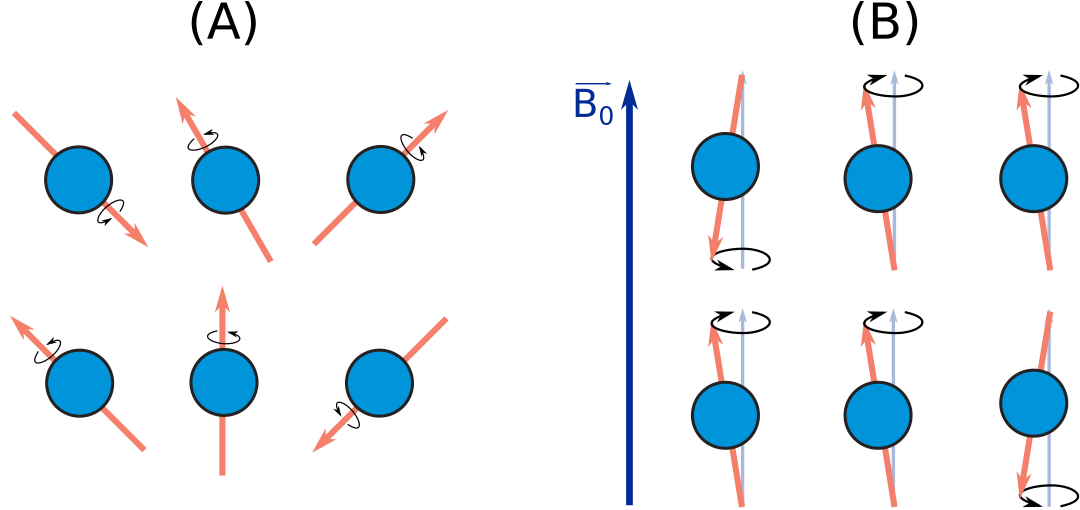
\includegraphics[width=0.49\textwidth]{3.mri/img/spin.png}
\caption{(A) When atomic nuclei rest under no constraints, they spins along
         random directions. (B) However, when putted under the effect of a
         magnetic field, the spin of the nuclei will align to the magnetic
         field's direction and start to precess around it.}
\label{fig:spin}
\end{figure} 

\section{Physics Background}

\subsection{Nuclear Magnetism}
\label{sec:nm}
Atomic nuclei with a different number of neutrons and protons are said to possess
a non-zero spin, which is an intrinsic form of angular momentum. While there is
not an actual movement, the nucleus spin can be interpreted as the particle 
spinning around its own axis~\cite{SEGALA1993}, since it possess all the same
physical properties. This "movement" of charges in the nucleus, induces what is
known as a nuclear magnetic moment (Fig. \ref{fig:spin} A).

When atomic nuclei are placed inside of an external magnetic field, their spin
will align with the field's direction and start to precess around it (Fig. \ref{fig:spin}) B).
While the spins could align either parallel or anti-parallel to the gradient, the
laws of thermodynamics ensure that a bigger number of spins will do it in the 
parallel direction.

The frequency with which the spin precess around the magnetic field is known 
as the Larmor frequency~\cite{Larmor1897}, and is expressed as:

\begin{equation}
    \label{eq:larmor}
    \omega = \vec{\mu} \times \vec{B} = \gamma \vec{J} \times \vec{B},
\end{equation}

where $\vec{\mu}$ is the magnetic moment of the nucleus; $\vec B$ is the
magnetic field; $\gamma$ is the gyromagnetic ratio of the atom, an intrinsic
physical property of each atom; and $\vec{J}$ is the angular momentum of the nucleus.

\begin{figure}[h]
    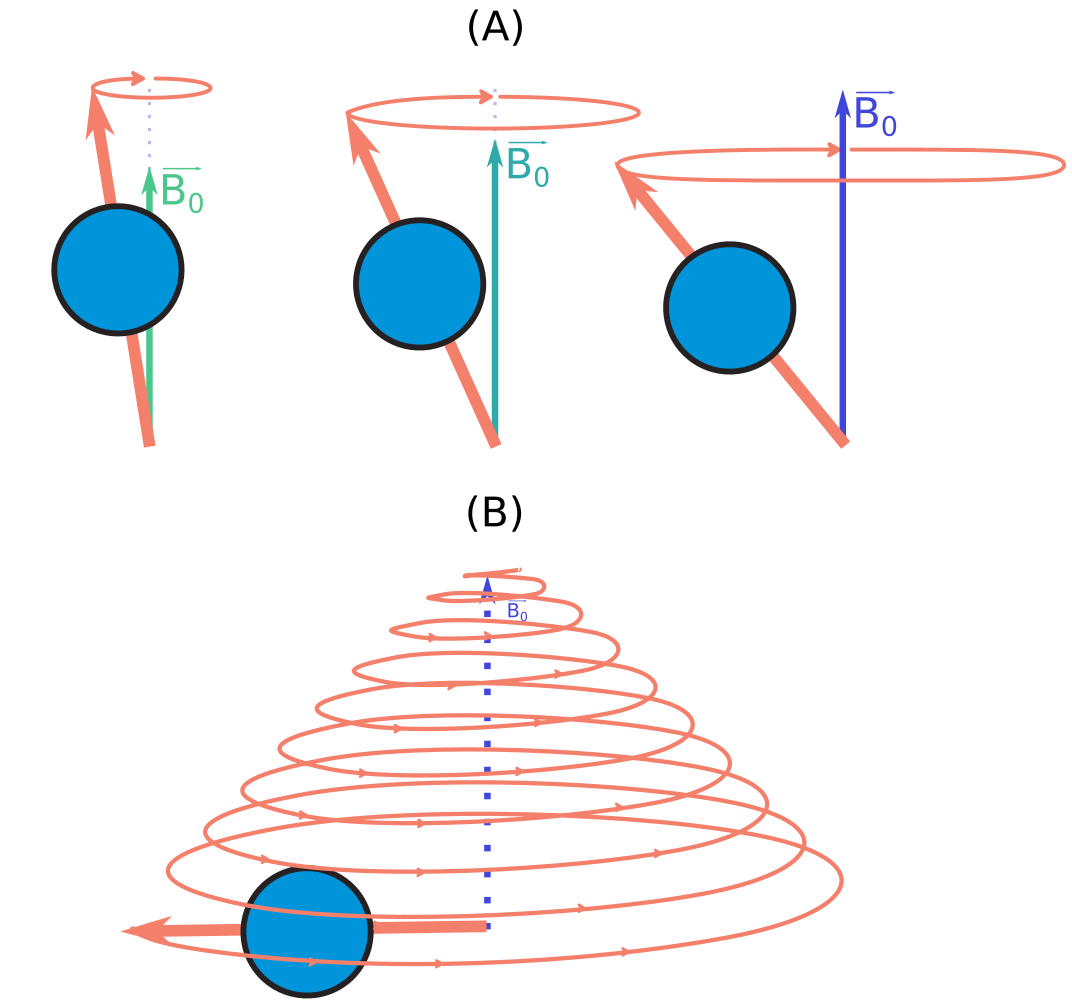
\includegraphics[width=0.49\textwidth]{3.mri/img/relaxation.png}
    \caption{(A) The higher the strength of the magnetic field, the bigger the angle
             between the nucleus spin and the magnetic field will be. (B) If the
             magnetic field ceases, the spin will return to its initial angle
             of precession.}
\label{fig:relaxation}
\end{figure} 

The angle formed between the precessing spin and the magnetic field is driven
by the strength of the magnetic field. The angle between the spin and the magnetic
field increases as the strength of the magnetic field does (Fig. \ref{fig:relaxation} A).
In fact, by increasing the energy of the magnetic field enough, it is possible
to 'excite' the nucleus, moving the precessing towards the plane transversal to
the magnetic field. However, if the external magnetic field
goes off, the nucleus will start to 'relax' (Fig. \ref{fig:relaxation} B), and
the precessing will begin to move once again towards the direction of the
magnetic field. An important remark is that the precessing angle does not
decrease linearly during the relaxation. This is because the relaxation
process represents a redistribution of the energy within the system. The energy that
the system won during excitation, has to go somewhere else in order for the
spin to go back to its initial state. In particular, spins lose energy by 
giving it to other non excited spin of the same kind (spin-spin interaction),
or by giving it to surrounding elements (spin-lattice interaction). This means
that how the relaxation happens is governed by the composition of the nucleus
itself, and the chemical composition of its environment. This process was
mathematically formalized by Bloch in what is known as the Bloch
Equations~\cite{Bloch1946}.

\subsection{Nuclear Magnetic Resonance}
The organs in the human body are composed by different types of tissue, each
with its own chemical composition. If we subject a human body to the effects
of excitation and relaxation by means of a magnetic field, and place a coil
in the transversal plane, we should be able to measure different relaxation
signals for different types of tissue. The problem is, that the amount of 
energy necessary to create a detectable precession would surely kill a human.
Another way to increment the energy of the system is needed, and for this is 
that the concept of Resonance is used.

Resonance is a physical phenomenon in which a system or external force drives
another system to oscillate with greater amplitude at specific frequencies.
In our case, we are interested in introducing more energy into the human body.
Knowing that hydrogen atoms ($^1 H$) are widely present in the body, we can
compute their Larmor frequency (Eq. \ref{eq:larmor}), and produce energy at
that frequency. By resonance, the produced energy will be injected into the
tissue.

\section{Nuclear Magnetic Resonance Imaging}

\begin{figure*}[t]
    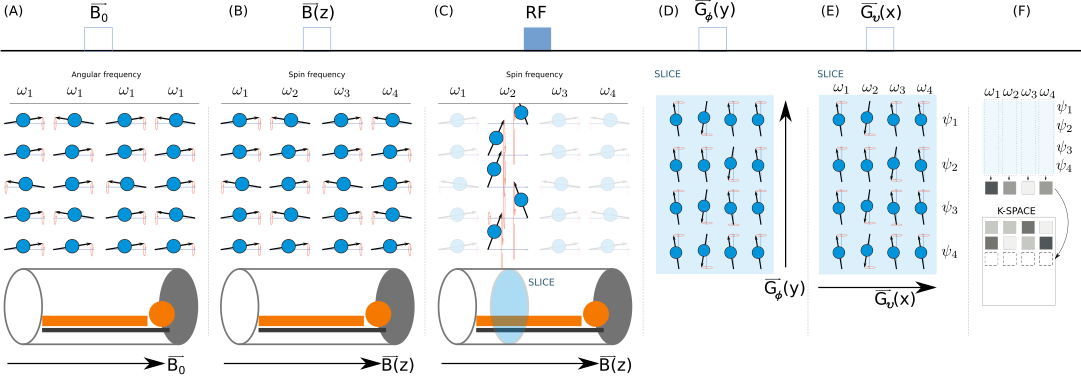
\includegraphics[width=\textwidth]{3.mri/img/mri.png}
    \caption{Simplified scheme of a MRI acquisition. (A) A MRI scanner is constantly
             emitting an homogeneous magnetic field $\vec B_0$ an atomic nuclei
             are precessing around it. (B) A gradient magnetic field is emitted
             in order to change in a predictable way the frequency of the nuclei.
             (C) A radio frequency pulse is generated, making certain nuclei to
             resonate and moving their precession to the transversal plane.
             (D) Now the slice is selected, a frequency encoding gradient is
             briefly applied to dephase nuclei in different vertical positions.
             (E) A phase encoding gradient is then turned on, to change in a predictable
             way the frequency in every horizontal position. (F) An acquisition
             is done and written down in the k-space.}
     \label{fig:mri}
\end{figure*}

Having covered the necessary physical notions, we are now ready to introduce
MRI. A MR scanner is a machine able to create strong magnetic fields and radio
frequency pulses in different frequencies. Particularly, while functioning
a MR scanner is constantly emitting an homogeneous magnetic field referred as $\vec B_0$
(Fig. \ref{fig:mri} A). If we place a coil in the plane transversal to $\vec B$,
and emit a radio frequency pulse at the frequency of hydrogen, we will be
able to measure a signal coming from the body. This measure will represent the
mixture of all the signals generated by different tissues. What we are interested
in, is to separate the signal coming from different places on the body, in order
to compare them after. A necessary first step to disentangle the different
contributions of each tissue is to do slice selection. 

Slice selection makes use of a gradient magnetic field. A gradient is a magnetic
field which strength varies linearly along a specific direction. Following the
Larmor equation (eq. \ref{eq:larmor}) we can predict that, nucleus along the
gradient will change their spin frequency in a predictable way. Particularly,
applying a gradient $B(z) \hat z$ in a specific direction (Fig. \ref{fig:mri} B),
will induce a frequency to the nuclei with magnetic momentum $\vec \mu$ of:

\begin{equation}
\label{eq:gradient}
    \omega(z) = \vec \mu \times B_z(z) \hat z.
\end{equation}

Then if a radio frequency (RF) pulse with a frequency of $w(z_0)$ is generated,
only the spins in the position $z_0 \hat z$ will start to resonate. Therefore,
the signal obtained by the transversal coil will only correspond to the spins in
the slice at position $z_0 \hat z $ (Fig. \ref{fig:mri} C) . It's important to state that, because of
hardware limitations, it's impossible to generate a RF pulse in an exact frequency.
What actually happens is that the pulse is generated for a small slice of
frequencies, meaning that the spins in a small band around $z_0$ will also
resonate.

So far, all of the spins inside of the slice are precessing in the same way.
We can think of the slice as a two dimensional matrix, with two coordinates:
$\hat x$ being the rows and $\hat y$ being the columns (Fig. \ref{fig:mri} B).
In order to retrieve the signal generated at each position, two more gradients
are needed, a frequency encoding gradient ($\vec G_{\nu}$) and a phase encoding
gradient ($\vec G_{\phi}$). 

First, $\vec G_{\phi}$ is applied for a short period of time in one of
the directions, lets say $\hat y$. Following the Larmor equation (eq. \ref{eq:larmor}),
all of the spins along $\hat y$ start to precess at a frequency that depends
on their position (Eq. \ref{eq:gradient}). After the gradient is shut down, the
spins will return to precess all at the same velocity, but off phase, since they 
where separated by the previous gradient. This is, the spins of each row will
have the same angular velocity, but a different phase (Fig. \ref{fig:mri} D).

Then, $\vec G_{\nu}$ is applied in the orthogonal direction ($\hat y$).
Now it will happen that: the spins of each row will be oscillating in a
different phase, because of $\vec G_{\phi}$ and the spins of each row will be
oscillating at a different velocity, following the new gradient $\vec G_{\nu}$
(Fig. \ref{fig:mri} E).

If we sample the signal using a coil over the direction $\hat x$, we will obtain
as many data points as columns. Each data point will have a mixture of all
the signals the rows (Fig. \ref{fig:mri} F).
However, each data point will comprise the difference in phase and the
difference in frequency that we applied to the matrix. By iteratively
measuring these data points, changing only the phase encoding gradient, we
sample what is known as the k-space\cite{Likes1981}. A space where the signal
generated by our sample is encoded by phase in the rows, and by frequency in the
columns. As shown by Likes et al.\cite{Likes1981}, taking the 2D Fourier
transform of the k-space, decodes the image of the tissue being sampled.

\section{Diffusion MRI}

\begin{figure*}[t]
    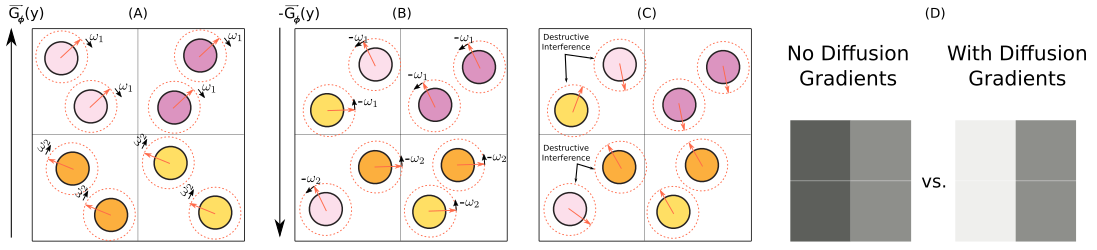
\includegraphics[width=\textwidth]{3.mri/img/diffusion.png}
    \caption{Simplified scheme of how diffusion is measured. We illustrated
             in the same plane as the gradient's direction so simplify the figure.
             (A) A first gradient field is applied, and the nuclei in the same
             rows start to precess in phase. (B) After some time, a gradient
             with the same strength is applied in the opposite direction. This
             gradient should cancel the phase shift induced by the first one.
             However, the particles undergoing diffusion would have change
             place. (C) Nuclei precessing at different phases will cause a
             destructive interference between them. (D) The off phase precessing
             is translated into lesser signal respect to the image acquired with
             no diffusion gradients.}
     \label{fig:diffusion_gradient}
\end{figure*}

While NMRI allows to visualize the different tissue composition of the brain,
diffusion MRI aims to quantify how the water molecules diffuse in the brain.
This is of great importance because in fibrous structure such as white matter,
water molecules tend to diffusion along fibers. Therefore, characterizing diffusion
can help to describe the underlying structure of the white matter. Now, we
start by explaining the phenomenon of diffusion and its implications in MRI.

\subsection{Brownian Motion and MRI}
The molecules inside a fluid in equilibrium are not still, on the contrary, 
they move randomly. This physical phenomena is known as Brownian motion~\cite{Brown1828}
or diffusion. In 1950, Hahn~\cite{Hahn1950} observes that the signal measured
during the relaxation period in MRI can be affected by the process of diffusion.

In order to characterize the effects of diffusion in nucleus relaxation, a
new experiment is devised. Imagine that after applying the RF pulse to do
slice selection, we apply two gradient fields (called diffusion gradients), one
after the other, with the same strength but in opposite directions (Fig. \ref{fig:diffusion_gradient} A).
As explained in section \ref{sec:nm}, this will induce two phase shifts to the nuclei.
The first gradient will make them go off phase, while the second one should
cancel the first, and put them back in phase. However, the particles undergoing
diffusion would have changed place, and therefore, change their phase differently
(Fig. \ref{fig:diffusion_gradient} B). Nuclei precessing at different phase on
a same sections of the sample will cause a destructive interference between them,
resulting in a lower signal. The ratio between the signal obtained with 
diffusion gradients and the one without them quantifies the amount of ongoing
diffusion (Fig. \ref{fig:diffusion_gradient} C).

In 1956, H.C. Torrey \cite{Torrey1956} extends the Bloch Equations~\cite{Bloch1946}
in order to quantify the effects of diffusion in nucleus relaxation when
multiple diffusion gradients are used. The new equations, known as Bloch-Torrey
equation cannot be solved analytically. It's not until 1965 that
Stejskal and Tanner~\cite{Stejskal1965} invent the Pulsed Gradient Spin
Echo (PGSE) sequence to measure diffusion in a specific direction. In their
sequence, two opposite diffusion gradients are applied for $\delta$ms, with a
separation of $\Delta$ms between them. If we assume $\delta$ to be infinitely
narrow (i.e. the diffusion during that time is negligible), then,
the Bloch-Torrey equations can be solved, and the signal attenuation at time
$2\tau = 2(\delta + \Delta)$  can be expressed as:

\begin{equation}
    E(2\tau) = 
    \frac{S(2\tau)}{S_0} =
    e^{-\gamma^2 g^2 \delta^2 \left(\Delta - \frac{\delta}{3}\right) D},
\label{eq:stejskal_tanner}
\end{equation}

where $g$ is the strength of the diffusion gradient, $S_0$ the
image acquired without diffusion gradients, and $D$ the diffusion coefficient.

\begin{figure}
    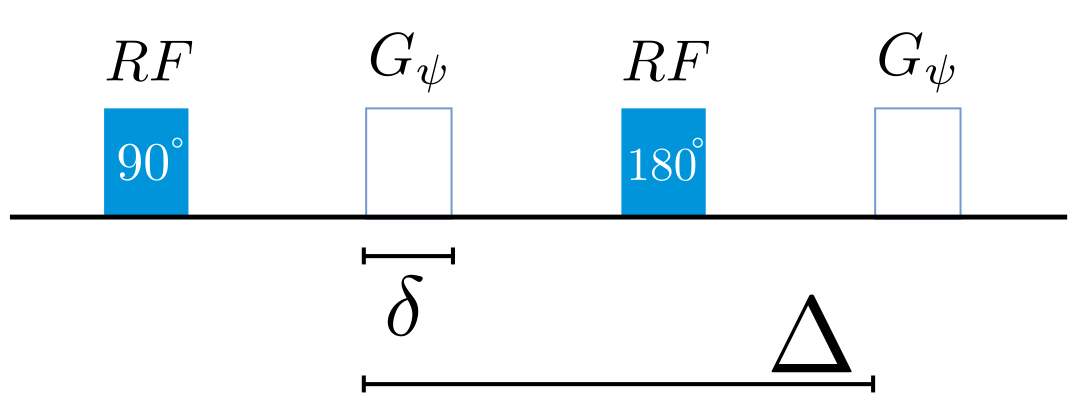
\includegraphics[width=0.49\textwidth]{3.mri/img/fgp.png}
    \caption{Pulsed Gradient Spin Echo sequence.}
    \label{fig:fgp}
\end{figure}  

In 1985 Le Bihan \cite{LEBIHAN} proposed to gather all the parameters in a
single one: 

$$ b = \gamma^2 g^2 \delta^2 \left(\Delta - \frac{\delta}{3}\right) $$ ,

simplifying the equation \ref{eq:stejskal_tanner} to:

$$ E(2\tau) = e^{-b D} $$

where $b$ has a physical meaning, it represents the reciprocal of the diffusion
intensity\cite{LEBIHAN}.

In 1991 Callaghan et al. \cite{Callaghan1991} developed the q-space analysis.
Based on the work of Stejskal and Tanner, Callaghan show that it's possible
to express the signal attenuation as:

\begin{equation}
\label{eq:callaghan}
E(q,\tau) =  \frac{S(q,\tau)}{S_0} = \int_{R^2}{P(r;\tau)e^{-2\pi i q r} dr},
\end{equation}

with $q =  \gamma \delta g / 2\pi$, and $P(r|r_0, \tau)$ a probability density
function (diffusion propagator) modeling the probability that a molecule had a
relative displacement of $r$ in time $\tau$. One of the main advantages of
q-space is that it does not assume any a prior model, allowing to define 
different strategies for $p(r;t)$. More importantly, equation
\ref{eq:callaghan} shows that the signal attenuation is the 3D Fourier
transform $\mathcal{F}$ of the average propagator $P$. 

\begin{equation}
    \label{eq:fourier_callaghan}
    E(q, \tau) = \frac{S(q, \tau)}{S_0} =
    \mathcal{F}[P(r|r_0, \tau)].
\end{equation}

In particular, if the diffusion propagator is assumed to be Gaussian, then the
Fourier integral can be solved analytically, and the solution is the same
as the one obtained by Stejskal and Tanner (Eq. \ref{eq:stejskal_tanner})

\begin{figure*}[h]
    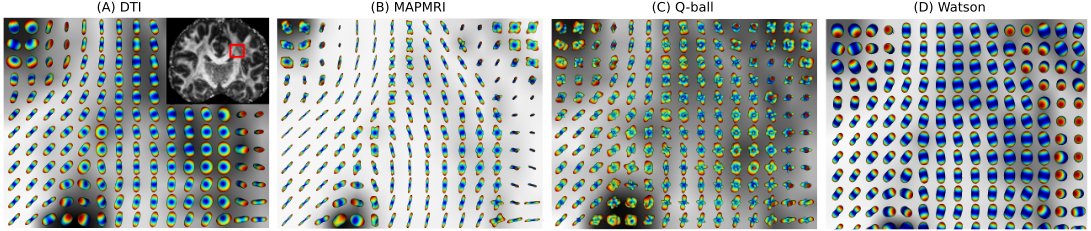
\includegraphics[width=\textwidth]{3.mri/img/models.png}
    \caption{Comparison of different models in the reconstruction of diffusion
             signal: (A) Diffusion Tensor Imaging, (B) Mean Apparent Propagator (MAP)-MRI,
             (C) Q-Ball Imaging, and (D) Watson distributions of NODDI. It can
             be seen that DTI finds an
             average orientation, where Q-Ball, MAPMRI and SMT find crossing
             structures. This image was adapted from Fick~\cite{Fick2017} (2017).}
     \label{fig:dwi_models}
\end{figure*}

\subsection{Diffusion Tensor Imaging (DTI)}
\label{sec:dti}
In 1994 Basser et al. \cite{Basser1994} propose to measure the signal attenuation
in different directions, and to model the diffusion coefficient in the Stejskal and
Tanner equation (eq. \ref{eq:stejskal_tanner}) with a second order tensor. This
sets the bases of what is known as Diffusion Tensor Imaging. DTI represents the
diffusion as a 3-dimensional (3D) ellipsoid, which can be coded in a symmetric
matrix:

$$
    D =
    \begin{pmatrix}
             D_{xx} & D_{xy} & D_{xz} \\
             D_{xy} & D_{yy} & D_{yz} \\
             D_{xz} & D_{yz} & D_{zz} 
    \end{pmatrix}.
$$

Since the matrix has 6 unknown variables, at least 6 acquisitions in different
directions have to be done. DTI is until today, one
of the most used techniques to model the diffusion signal. Its main drawback
is that it does not allow to correctly characterize the crossing of fibers. Both
the isotropic diffusion and the crossing of fibers get modeled as spheres.

\subsection{High Angular Resolution Diffusion Imaging}
\label{sec:hardi}
Two factors drive newer imaging techniques: Callaghan's relationship~\cite{Callaghan1991}
between the signal attenuation and the diffusion propagator 
(Eq. ~\ref{eq:fourier_callaghan}), and the ability to acquire data across many
different angles with different b-values. Either using one b-value (singel shell)
or multiple b-values (multi shell), HARDI techniques rely on taking acquisitions
across many different angles, in order to reconstruct the true diffusion propagator.
Notable examples of High Angular Resolution Diffusion Imaging (HARDI) are Diffusion
Spectrum Imaging (DSI)~\cite{Wedeen2008}, Q-space Imaging (QSI)~\cite{Callaghan1991},
Q-Ball Imaging~\cite{Tuch2004}, Composite hindered and restricted model of diffusion (CHARMED)~\cite{Assaf2005},
Mean Apparent Propagator (MAP)-MRI~\cite{Ozarslan2013}, 
Constrained Spherical Deconvolution~\cite{Tournier2004}, and Neurite
Orientation Dispersion and Density Imaging ( NODDI~\cite{Zhang2012}. While each technique
relies in different assumptions about the diffusion propagator,
they all try to capture multiple fiber directions within the same imaging
voxel. HARDI acquisitions are currently being improved every day with better 
material and better reconstruction algorithms.

\subsection{Estimating Axonal Connectivity}
So far, we discussed about imaging techniques to measure diffusion. Now is time
to present how to use such techniques in order to study the structure of white matter.

Water particles in the white matter diffuse constrained by the axonal bundles.
The nuclei present at any point of the white matter will be able to diffuse
only inside a tract and along its path. If dMRI had enough resolution, we
could trace each brain connection by simply looking at the diffusion signal.
However, this is not the case, dMRI resolution is several orders of magnitude
coarser than axonal diameters (millimeters vs micrometers)~\cite{VanEssen2014}.
What is done in practice, is to fit one of the models named in previous sections
(sec. \ref{sec:dti}, \ref{sec:hardi}), and use them to derive a probabilistic
map of transition from each voxel to their neighbors. The resulting network can
be used on a Monte Carlo procedure where, starting from a voxel, at each step we
randomly select to which neighboring voxel to move, following the
probabilistic map. This process of simulating the random walk of a water
particles through the white matter is known as Tractography~\cite{Behrens2003a}.

The field of tractography is not exempt of problems, most state state-of-the-art
algorithms create about four time more false‐positive tracts than true‐positive
ones~\cite{Maier-hein2017}. Also, most of them suffer from gyral bias, in which tractography bundles
are biased towards finishing in gyral crowns rather than sulcal banks~\cite{VanEssen2014}.
However, tractography has shown to be able to recover some major
bundles in humans~\cite{Catani2008}. Also, it has been validated using high-resolution
postmortem diffusion imaging and tractography in Old World monkeys. Particularly,
Donahue et al.\cite{Donahue2016} found a correlation
coefficient of ~0.58 between tractography-based and tracer-based estimates of
connectivity; the correlation is highest for strong, short-distance pathways
but is informative even for weak connections and widely separated areas. This
results, encourage to use tractography, despite of its flaws.

\section{Brief Introduction to Functional MRI}

Built on the contributions of Pauling and Coryell~\cite{Pauling1936}, and 
Ogawa\cite{Ogawa1990, Ogawa1993} among others, functional MRI (fMRI) characterizes
blood flow in the brain. Since blood flow is directly related with brain
activity, fMRI gives us a way to study brain function. While not central to our
thesis, we do believe that at least a brief description of how functional MRI
(fMRI) works should be given.

When a region of the brain is activated by a cognitive task, the local firing
of neurons generates a higher energy requirement~\cite{Glover2011}.
The brain responds by adjusting its blood supply to the region in a process
known as the haemodynamic response. This increase in blood flow produces an
increase in the ratio of oxygenated hemoglobin relative to deoxygenated hemoglobin
in that specific area (BOLD contrast). Oxygenated hemoglobin is magnetically 
indistinguishable from brain tissue. On the contrary, deoxygenated hemoglobin
has 4 unpaired electrons and is highly paramagnetic\cite{Glover2011}. This
results in local gradients that dephase the nuclei around it, causing destructive
interference in the observed MR signal. Using a special type of pulse sequence
called gradient refocused echo~\cite{Elster1993} it is possible to make MR
scanners sensible to this effect.

After obtaining the fMRI signal, it is possible to estimate which brain regions
are being more active during the desired cognitive task by means of statistics.
In particular, it is expected to see a high activation of the area being used
for a task while the subject is doing such task. For example, in order to
obtain the area to finger movement, we could ask a subject to start and stop
moving the finger at regular intervals. The area responsible for moving the
finger should show a regular activation pattern, correlated with the moments
in which the finger was moving. We can compute such area by selecting the voxels
in which the fMRI signal correlates the most with the square signal of finger
movement (1 when the finger was moving, 0 when not).

\section{Conclusion}
This chapter introduced the imaging techniques of MRI, Diffusion MRI and
Functional MRI. These three methods provide means to study the brain anatomy,
its axonal organization and function in a non-invasive way. Even when each
technique has its own limitations, either in spatial or temporal resolution,
they all allowed to highly advance the state of the art in neuroscience. In
the next chapter we will see how these advances in imaging allowed to parcellate
the brain, making it easier to study brain function.

\chapterbib


%In 1946, Bloch \cite{Bloch1946} introduce phenomenological equations that explain
%shows that the variation in magnetization over
%time for a nucleus is expressed as:


%%Where $\gamma$ is the gyromagnetic ratio, $B$ is the magnetic field intensity and T1, T2 are relaxation times.
%In 1950, Hahn~\cite{Hahn1950} observes that the signal measured during
%the relaxation period in MRI can be affected by the process of diffusion.
%In 1956, H.C. Torrey \cite{Torrey1956} presents phenomenological equations that
%incorporate this effect to the Blochs equation, creating the Bloch-Torrey equation:
%
%\begin{equation}
%    \label{eq:block_torrey}
%    \frac{dM}{dt} = \\
%    \gamma M \times B_0 
%    + \left( \frac{M_x}{T_2}, \frac{M_y}{T_2}, \frac{M_0-M_z}{T_1} \right)
%    + D\bigtriangledown^2M.
%\end{equation}

%Here, $M$ is the magnetization of an excited sample placed in a static magnetic
%field $B_0$, $\gamma$, is the gyromagnetic ratio, $M_x$, $M_y$, $M_z$ are the 
%components of magnetization in the x, y and z directions, $M_0$ is the magnetization
%at thermal equilibrium, $T_1$ and $T_2$ are relaxation times and $D$ is a diffusion
%coefficient. The first two terms of equation \ref{eq:block_torrey} are the original
%Bloch equation~\cite{Bloch1946}. The third term of equation \ref{eq:block_torrey}
%was added by Torrey.
